\label{cha:larch}
To simultaneously learn a latent representation of cellular gene expression data and their hierarchical relationships, a tree-structured topic model is introduced. In this chapter, details of this model, referred to as a \underline{La}tent \underline{R}epresentation of \underline{C}ellular \underline{H}ierarchies (LaRCH), are shown along with the results of a trained model on a simulated single-cell gene expression dataset. 

\section[LaRCH]{LaRCH: \underline{La}tent \underline{R}epresentation of \underline{C}ellular \underline{H}ierarchies}

\begin{figure}
    \centering
    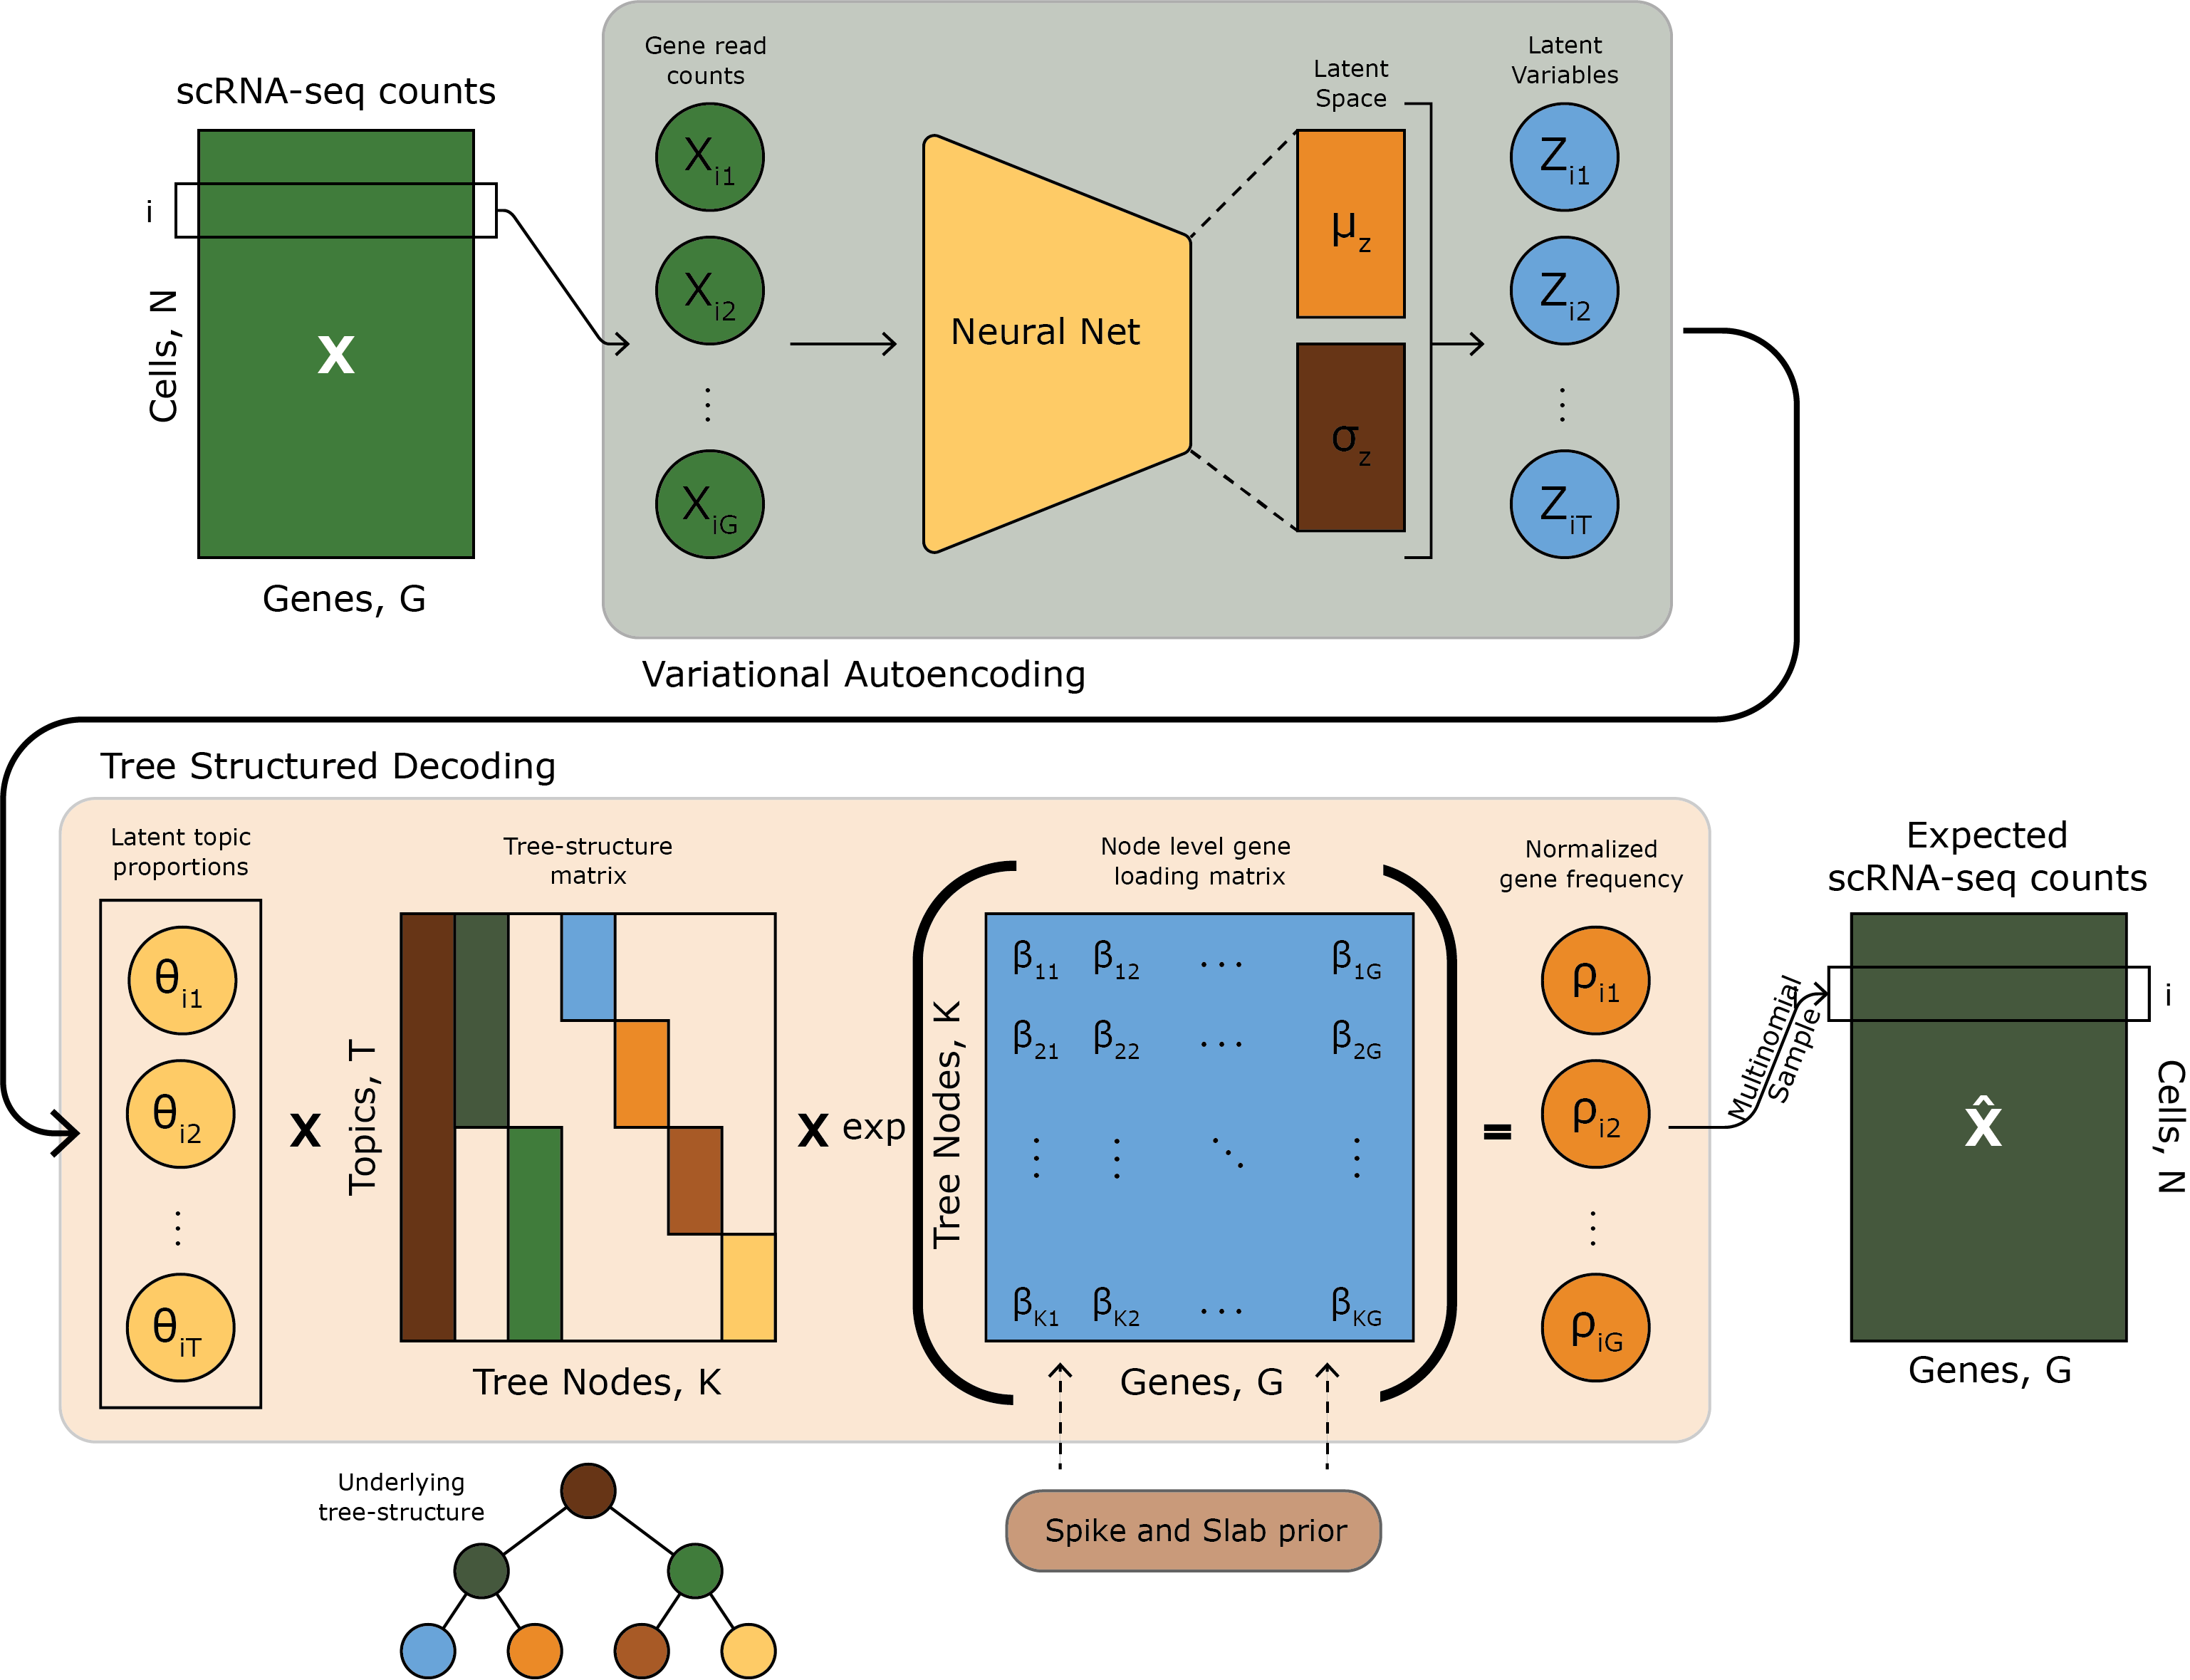
\includegraphics[width=\textwidth]{Figures/LaRCH_overview_0.png}
    \caption{\textbf{Overview of the LaRCH method} scRNA-seq data is encoded in latent features using a VAE. Original input data is then reconstructed through a generalized linear decoder containing the underlying PBT structure.}
    \label{fig:LaRCH}
\end{figure}

LaRCH uses an ETM \cite{etm1} approach built on a VAE \cite{Kingma2013-if,Kingma2014-pp,Kingma2015-mo} framework borrowed from neural network architectures with additional tree-node layer that aggregates sparse gene expression effects. Within a typical ETM, cells are represented as a mixture of latent topics each describing a gene expression profile of raw scRNA-seq count data. LaRCH introduces an additional layer of latent nodes that lie within a PBT structure (Fig. \ref{fig:LaRCH}). As a result, cells are viewed as a mixture of latent topics, each corresponding to a summation of tree nodes along a path from the root node to a given leaf node of the underlying tree. From this structure, it is inferred that topics that lie in close proximity on the tree share a number of properties while those further apart are also more distant in their features. As a more specific example, two topics corresponding to paths terminating at sibling leaf nodes would share all features captured in their common parent nodes, only diverging at the last branching point in their paths. Cells within these two topics would be said to share a large number of gene expression features represented by their shared parent nodes in their topic paths. 

The LaRCH model is comprised of an encoder and decoder component. The encoder transforms raw single-cell gene expression count data into the latent topic space through a neural net. In this model, rather than choosing the number of latent topics to represent the data, the depth of the latent-node tree $D$ is pre-determined, therefore the resulting number of total latent tree nodes is $2^D - 1$, and the latent topic space that the gene count data is transformed to is of dimension $2^{D-1}$. This latent representation is then converted to a topic proportion representation using the softmax function. 

Where LaRCH differs from a typical ETM lies in the decoder. The decoder contains a gene embedding matrix $\beta$ for each tree node as model parameters. Gene embedding values represent relative gene expression frequencies for a given tree node. Additionally, the tree-structured relationships at the topic level are represented mathematically using a structural matrix. The learned gene embedding matrix, structural matrix, and inferred topic proportions are passed to a GLM to estimate the cell specific gene frequencies for each data point. These gene frequencies are then used to compute likelihood values for expected gene counts.


\subsection{Data generative scheme}

To apply the LaRCH topic model, each cell is treated as a document, the set of genes in the dataset as the vocabulary of size $G$, and each scRNA-seq read as a token of a gene from the vocabulary. Each cell $i$ of $N$ cells is then represented as a mixture of $T$ latent topics in our model. 

In a classic ETM, each topic has a corresponding distribution over the gene space $\beta \in \mathbb{R}^{T \times G}$ \cite{etm1}. This is altered by introducing an additional latent tree node layer to the embedding process. $K$ latent nodes lie in a PBT structure of depth $D$, where $K = 2^D - 1$. Each of the $T$ latent topics, where $T = 2^{D-1}$, corresponds to a path from the root node to a leaf node of the PBT. Each tree node now has an embedding over the gene space $\beta \in \mathbb{R}^{K \times V}$ and each topic also has an embedding made up of the tree nodes along its corresponding path $\bar{\beta} =A\exp(\beta)$, where $A$ is a $T \times K$ matrix that captures the PBT structure. From this, two topics with similar paths in the tree-structured node will share gene embeddings while the paths are identical, then differ once the paths split. 

The formal data-generating process for each cell $i$, where $i = 1, \dots, N$, in the scRNA-seq dataset is:
\begin{enumerate}
    \item Draw latent topic proportion $\theta_i$ for cell $i$ from:
    \begin{equation}
        \theta_i = \text{softmax}(z_i) = \frac{\exp(z_{it})}{\sum_{t = 1}^T \exp(z_{it})}, z_i \sim \mathcal{N}(0, \textbf{I})
    \end{equation}
    \item Determine the categorical distribution $\rho_i$ of genes for cell $i$ based on $\theta_i$:
    \begin{equation}
        \tilde{\rho}_i = \theta_iA\exp(\beta), \rho_i \sim \text{Dirichlet}(\tilde{\rho}_{i1}, \tilde{\rho}_{i2}, \dots, \tilde{\rho}_{iG})
    \end{equation}
    \item Draw gene $g$ for each read of a cell from a multinomial distribution to give total gene counts over $R$ reads:
    \begin{equation}
        X_i|\rho_i \sim \text{Multinomial}(R, \rho_i)
    \end{equation}
    This gives the probability distribution: 
    \begin{equation*}
        p(X_i|\rho_i)\propto \prod_{g\in G} \rho_{ig}^{X_{ig}}
    \end{equation*}
    Where $\sum_{g}\rho_{ig} = 1$ for all $i \in 1, \dots, N$ and $\rho_{ig} \geq 0$ for all cells $i$ and genes $g \in [G]$
\end{enumerate}

Gene expression counts are said to follow independent multinomial probabilities (a bag of words assumption). Compared to other deep learning methods based on Poisson, Negative Binomial, and Gaussian distributions, a multinomial likelihood better preserves scale-invariant properties mitigating batch effects on the trained model. 

Here $z_i$ is the $1 \times T$ latent topic embedding of cell $i$, $\theta_i$ is the $1 \times T$ topic mixture of cell $i$ where $\sum_{t = 1}^T\theta_{i,t} = 1$, $\beta$ is a $K \times G$ gene embedding matrix for latent nodes, $A$ is a $T \times K$ matrix representing the tree-structure of nodes, $\rho_i$ is the $1 \times G$ cell specific distribution of gene reads, and $X_i$ is the $1 \times G$ count vector of genes. 

\subsection{Informing Model Parameters Through Bayesian Priors}
\subsubsection{A Dirichlet Prior to Inform Multinomial Sampling}

A Dirichlet prior is introduced to inform the categorical distribution of genes for each given cell, $\rho_i \sim \text{Dir}(\tilde{\rho}_i)$. This allows for direct transformation from the parameters $\tilde{\rho}$ to a distribution vector from which to sample multinomial values. The Dirichlet parameters are formulated as a GLM,
\begin{equation*}
    \tilde{\rho}_{ig} = \sum_{t = 1}^T\theta_{it}\sum_{k = 1}^K A_{tk}\exp(\beta_{kg}) - Db_g
\end{equation*}

This GLM captures the additive effects of nodes within each topic and the proportional additive effects of topics within each cell on the relative gene expression profile. 

An additional gene-specific bias parameter $b_g$ is used to represent invariant effects across all latent nodes. Since this parameter is present for each node, at the topic level, the additive effect of this parameter is $Db_g$. This is a free parameter without any specified prior distribution.
 
Since the multinomial and Dirichlet distribution share a conjugate relationship, the composite variable $\rho$ can be integrated out to obtain the posterior predictive likelihood, 
\begin{align*}
    p(x_i | \theta_i, \{\beta_{kg}\}, \{b_g\}) &= \int p(x_i | \rho_i)p(\rho_i | \theta_i, \{\beta_{kg}\}, \{b_g\})d\rho_i\\
    &= \frac{\Gamma(\sum_g \tilde{\rho}_{ig})\Gamma(\sum_g X_{ig} + 1)}{\Gamma(\sum_g \tilde{\rho}_{ig} + X_{ig})}\prod_g\frac{\Gamma(X_{ig} + \tilde{\rho}_{ig})}{\Gamma(\tilde{\rho}_{ig}) \Gamma(X_{ig} + 1)}\\
    &\propto \frac{\Gamma(\sum_g X_{ig} + 1)}{\prod_g \Gamma(X_{ig} + 1)}\frac{\prod_g\Gamma(X_{ig} + \tilde{\rho}_{ig})}{\Gamma(\sum_g \tilde{\rho}_{ig} + X_{ig})},
\end{align*}

where $\tilde{\rho}_{ig} = \sum_{t = 1}^T\theta_{it}\sum_{k = 1}^K A_{tk}\exp(\beta_{kg}) - Db_g$, and $\Gamma(\cdot)$ is the Euler's gamma function.

\subsubsection{Using a Bayesian Prior to Induce Model Sparsity}
Since scRNA-seq data is typically sparse with only a few non-zero features and shared expression of many highly expressed genes in general, the trained model used to represent this data should reflect this. To induce sparsity and increase interpretability in the gene embedding model parameters, $\beta$, a Bayesian spike-and-slab distribution prior \cite{Mitchell1988-yj} is used to inform their values. Within the spike-and-slab prior distribution, it is assumed that the majority of gene-embedding values $\beta_{kg}$ are statistically zero with some probability $1-\pi$. This concentration around zero is called the "spike" component of the distribution. The "slab" portion of the distribution is explained by a normal distribution centred around 0 with variance $\tau$. 
\begin{equation}
    \beta_{kg} \sim \pi \mathcal{N}(0,\tau) + (1 - \pi)\delta_0 (\beta_{kg})
\end{equation}




\subsection{Variational Inference}
Since exact inference of the posterior probability of latent topics $p(\theta_i | x_i)$ is computationally intractable in high dimensional spaces, stochastic variational inference is used as a scalable approach to finding approximate distributions \cite{Kingma2013-if}. 

The variable estimation scheme as described in Kingma \textit{et al.} is used\cite{Kingma2013-if}. In this reparameterization technique, latent variable inference is cast into an optimization problem in a deep belief network. This can then be solved using back-propagation steps with respect to model parameters. 

Variational inference is used to estimate two sets of parameters, the cell-specific latent topic proportions $q(\theta_n)$ and the node-specific gene-embedding parameters $q(\beta_{kg})$. For each set of parameters, the minimized Kullbeck-Leibler (KL) divergence is used to approximate the actual data likelihood probability. This is equivalent to maximizing the evidence lower bound (ELBO) for the total data likelihood, $\mathcal{L}$.

\begin{align}
    \ln p(\textbf{X}) & \geq 
    \mathbb{E}_q \left[\ln \frac{ p(\textbf{X}, \Theta, \beta)}{q(\Theta, \beta | \phi, \xi)}\right] \triangleq \mathcal{L}\\
    \sum_{i\in [N]}\int_{\theta, \beta}p(x_i, \theta_i, \beta) d\theta_i d\beta_i & \geq\mathbb{E}_q\left[\ln \frac{p(\textbf{X} | \Theta, \beta) p(\theta_i) p(\beta | \pi, \tau)}{q(\Theta | \phi)q(\beta | \xi)}\right]    \\
     \label{ELBO} = \mathbb{E}_q\left[\sum_{i\in [N]}\ln p(x_i | \theta_i, \beta)\right] &+ \mathbb{E}_q \left[\sum_{i\in [N]} \ln \frac{p(\theta_i)p(\beta | \pi, \tau)}{q(\theta_i|\phi)q(\beta|\xi)}\right] \\ 
     = \mathbb{E}_q \left[\sum_{i\in [N]}\ln p(x_i | \theta_i, \beta)\right] &+ \sum_{i\in [N]} \left[ \mathbb{E}_q \left[\ln \frac{p(\theta_i)}{q(\theta_i|\phi)}\right] + \mathbb{E}_q \left[\ln \frac{p(\beta | \pi, \tau)}{q(\beta|\xi)}\right]\right]\\
     \label{KL-elbo} = \mathbb{E}_q \left[\sum_{i\in [N]}\ln p(x_i | \theta_i, \beta)\right] &- \sum_{i\in [N]} \left[\text{D}_{\text{KL}}(q_\theta \parallel p_\theta) + \text{D}_{\text{KL}} (q_\beta \parallel p_\beta)\right]
\end{align}

Where $\phi$ and $\xi$ are used to denote all parameters of the latent state or parameter distributions, $\pi$ and $\tau$ are the probability of inclusion and variance parameters, respectively. Stochastic gradient steps with respect to the variational parameters $\phi$ and $\xi$ are taken in the variational inference algorithm, optimizing the ELBO objective (\ref{ELBO}) in order to find approximate posterior distributions. Variational inference is implemented in \texttt{Pytorch} using \texttt{torch.autograd} \cite{pytorch, pytorchdiff} to calculate gradients. 

\subsubsection{Approximation of latent topic proportions $\theta$}

Latent topic proportions, $\theta$ cannot be exactly evaluated, so are instead approximated by summing over the posterior predictive log-likelihood using sampled instances of $\theta^{(s)}$ and $\beta^{(s)}$ for each minibatch sample $s \in [S]$

\begin{equation}
    \mathbb{E}_q \left[\sum_{i\in [N]} \ln p(x_i|\theta_i, \beta)\right] \approx \frac{1}{S} \sum_{s \in [S]} \ln p(x_s | \theta^{(s)}, \beta^{(s)})
\end{equation}

The mean $\mu$ and variance $\sigma$ functions for latent variable inference are parameterized in the encoder model which takes the original high-dimensional scRNA-seq data $x$. $\theta^{(s)}$ is then posteriorly sampled using the reparameterization trick of the Logistic Normal distribution as follows: 
\begin{enumerate}
    \item Sample random error $\epsilon_s \sim \mathcal{N}(0,1)$
    \item Reparameterize latent topic variables $z_s \leftarrow \mu(x_s) + \sigma(x_s) \circ \epsilon_s$
    \item Transform latent variables to latent topic proportions: \\$\theta_t^{(s)} \leftarrow \frac{\exp(Z_{st})}{\sum_{j = 1}^T \exp(Z_{sj})}$
\end{enumerate}

Assuming $z_s \sim \mathcal{N}(0, I)$ \textit{a priori} for all $s$, the corresponding variational parameters $\phi \equiv (\mu, \sigma)$ is used to derive the KL divergence between the prior and variational distributions as the second term of (\ref{KL-elbo}): 
\begin{equation}
    \mathbb{E}_q \left[\ln \frac{q(Z_{st} | \phi)}{p(Z_{st})}\right] = \text{D}_{\text{KL}}(q_\theta \parallel p_\theta) = \sum_{t = 1}^T \frac{1}{2}[\mu_{st}^2 + \sigma_{st}^2 - \ln \sigma_{st}^2 - 1]
\end{equation}

\subsubsection{Approximation of global spike-and-slab parameters $\beta$}

Fully-factored spike-and-slab distributions are used as variational distributions for node-specific gene embedding parameters, $\beta_{kg}$, to derive the final term of (\ref{KL-elbo}), the negative KL loss of the global parameters, $\beta$.

When $\beta_{kg}$ is 'on', denoted by a latent indicator variable $h_{kg} = 1$ with probability $\alpha_{kg}$, $\beta_{tg}$ is parameterized by a Gaussian distribution:

\begin{equation*}
    q(\beta_{kg}| h_tg =1) = \mathcal{N}\left(\mu_{kg}^\beta, \nu_{kg}^\beta\right)
\end{equation*}

with probability $\alpha_{kg} \triangleq p(h_{kg} = 1)$; otherwise, $\beta_{kg}$ is set to zero:
\begin{equation*}
    q(\beta_{kg}|h_{kg} = 0) = \delta_0(\beta_{kg})
\end{equation*}

with probability $1-\alpha_{kg}$.

From the variational parameters $\xi \equiv (\alpha, \mu, \nu)$, the variational distribution is characterized as:

\begin{equation}
    q(\beta_{kg}) = \prod_{g\in G} \alpha_{kg}\mathcal{N}(\mu_{kg}, \nu_{kg})
\end{equation}

with 

\begin{equation}
    \mathbb{E}_q[\beta_{kg}] = \alpha_{kg}\mu_{kg} \label{eq:betahat_est} 
\end{equation}
\begin{equation}
    \mathbb{V}_q[\beta_{kg}] = \alpha_{kg}(1-\alpha_{kg})\mu_{kg}^2 + \alpha_{kg}\nu_{kg} \label{eq:betahat_var}
\end{equation}

This give the full reparameterization of $\beta$ as follows:
\begin{enumerate}
    \item Sample random error $\epsilon\sim\mathcal{N}(0,1)$
    \item Reparameterize node-specific gene embedding values $\beta_{kg} \leftarrow \mathbb{E}_q[\beta_{kg}] + \mathbb{V}_q[\beta_{kg}]^{\frac{1}{2}}*\epsilon - b_g$
\end{enumerate}

Assuming $h_{kg} = 1$ with probability $\pi_0$ and $\beta|h=1 \sim \mathcal{N}(0, \tau_0)$ \textit{a priori}, the KL loss is derived as follows:

\begin{align}
    -D_{KL}(q||p) = &\frac{\alpha_{kg}}{2}\left[1 + \ln \frac{\nu_{kg}}{\tau_0} - \frac{1}{\tau_0}(\mu_{kg}^2 + \nu_{kg})\right] + \\
    &\left[\alpha_{kg}\ln\frac{\pi_0}{\alpha_{kg}} + (1 - \alpha_{kg}\ln\left(\frac{1 - \pi_0}{1 - \alpha_{kg}}\right)\right]
\end{align}

\subsection{Model Implementation}

LaRCH is implemented in Python, using the \texttt{PyTorch} machine learning library \cite{pytorch}. The model makes use of the \texttt{torch.autograd} function to perform stochastic variaitonal inference \cite{pytorchdiff}.

\subsection{Code Availability}

Code containing the most up-to-date version of the \texttt{LaRCH} package, documentation, data simulation scripts of the simulation scheme presented in \ref{cha:datasim}, and a model pipeline can be found at \url{https://github.com/causalpathlab/LaRCH}.

\newpage
\section[Modeling Simulated Data]{Modeling Simulated Data from Bulk RNA-seq Expression}

Simulated single-cell gene expression data of immune cell subtypes was generated based on bulk-sequenced gene expression profiles from the Database of Immune Cell Expression \cite{DICE1}. This generated data was then used to train an instance of the LaRCH model in order to test its efficacy. 

\subsection{Bulk Gene Expression Profile Generation}
The DICE database bulk gene expression profiles are measured from human PBMCs obtained from leukapheresis samples. Immune cell types of interest were isolated from PBMC samples prior to total RNA isolation using fluorescence-activated cell sorting (FACS) based on fluorescent antibody staining either directly or following pre-enrichment using human B cell or memory CD4+ T cell isolation kits for B cell and CD4+ T cell samples, respectively \cite{DICE1}. FACS-sorted naive CD4+ and CD8+ T cells underwent an additional \textit{ex vivo} CD3/CD28 activation step for their respective activation conditions. 

Total RNA purified from FACS-sorted cell samples was then bulk sequenced and mapped against the hg19 reference genome and the GENCODE annotation v19 as the gene reference model. The expression profiles used in the data simulation scheme are expressed in transcripts per million (TPM) units. A full outline of the sample processing and RNA sequencing steps for this data can be found in Schmiedel et al. \cite{DICE1}.



\subsection{Data Simulation Scheme}
\label{cha:datasim}
The simulation scheme used to generate realistic single-cell gene expression data for $N$ cells is as follows:
\begin{enumerate}
    \item Determine the desired noise proportion $\rho$ and total transcript count $R$. $\rho$ represents the proportion of the gene expression distribution for a given 'cell' that is explained by a null distribution, $\pi_0$, common to all cell types. $1-\rho$ then represents the proportion of the gene expression distribution for a given 'cell' that is explained by a cell-type specific distribution $\hat{\pi}_t$. 
    \item Determine the null and cell type-specific gene expression distributions, $\pi_0$ and $\hat{\pi}$, respectively:
    \begin{equation}
        \pi_0 \sim \text{Dirichlet}(1, \dots, 1), 
        \hat{\pi}_{tg} = \frac{\text{bulk}_{tg}}{\sum_g \text{bulk}_{tg}}
    \end{equation}
    Where bulk$_{tg}$ is the bulk expression profile for cell type $t$ at gene $g$.
    \item Determine a cell type distribution across the simulated data sample, $m$:
    \begin{equation*}
        m \sim \text{Dirichlet}(1,\dots, 1)
    \end{equation*}
    \item For a cell $i$, where $i = 1, \dots, N$:
    \begin{enumerate}
        \item Randomly sample cell type $t_i$ according to $t_i \sim \text{Categorical}(m)$
        \item Gene expression distribution for cell type $t_i$:
        \begin{equation}
            \pi_{t_i} = (1 - \rho) * \hat{\pi}_{t_i} + \rho * \pi_0
        \end{equation}
        \item Sample gene transcript counts $X_i$:
        \begin{equation*}
            X_i \sim \text{Multinomial}(R, \pi_t)
        \end{equation*}
    \end{enumerate}
\end{enumerate}


\begin{figure}
    \centering
    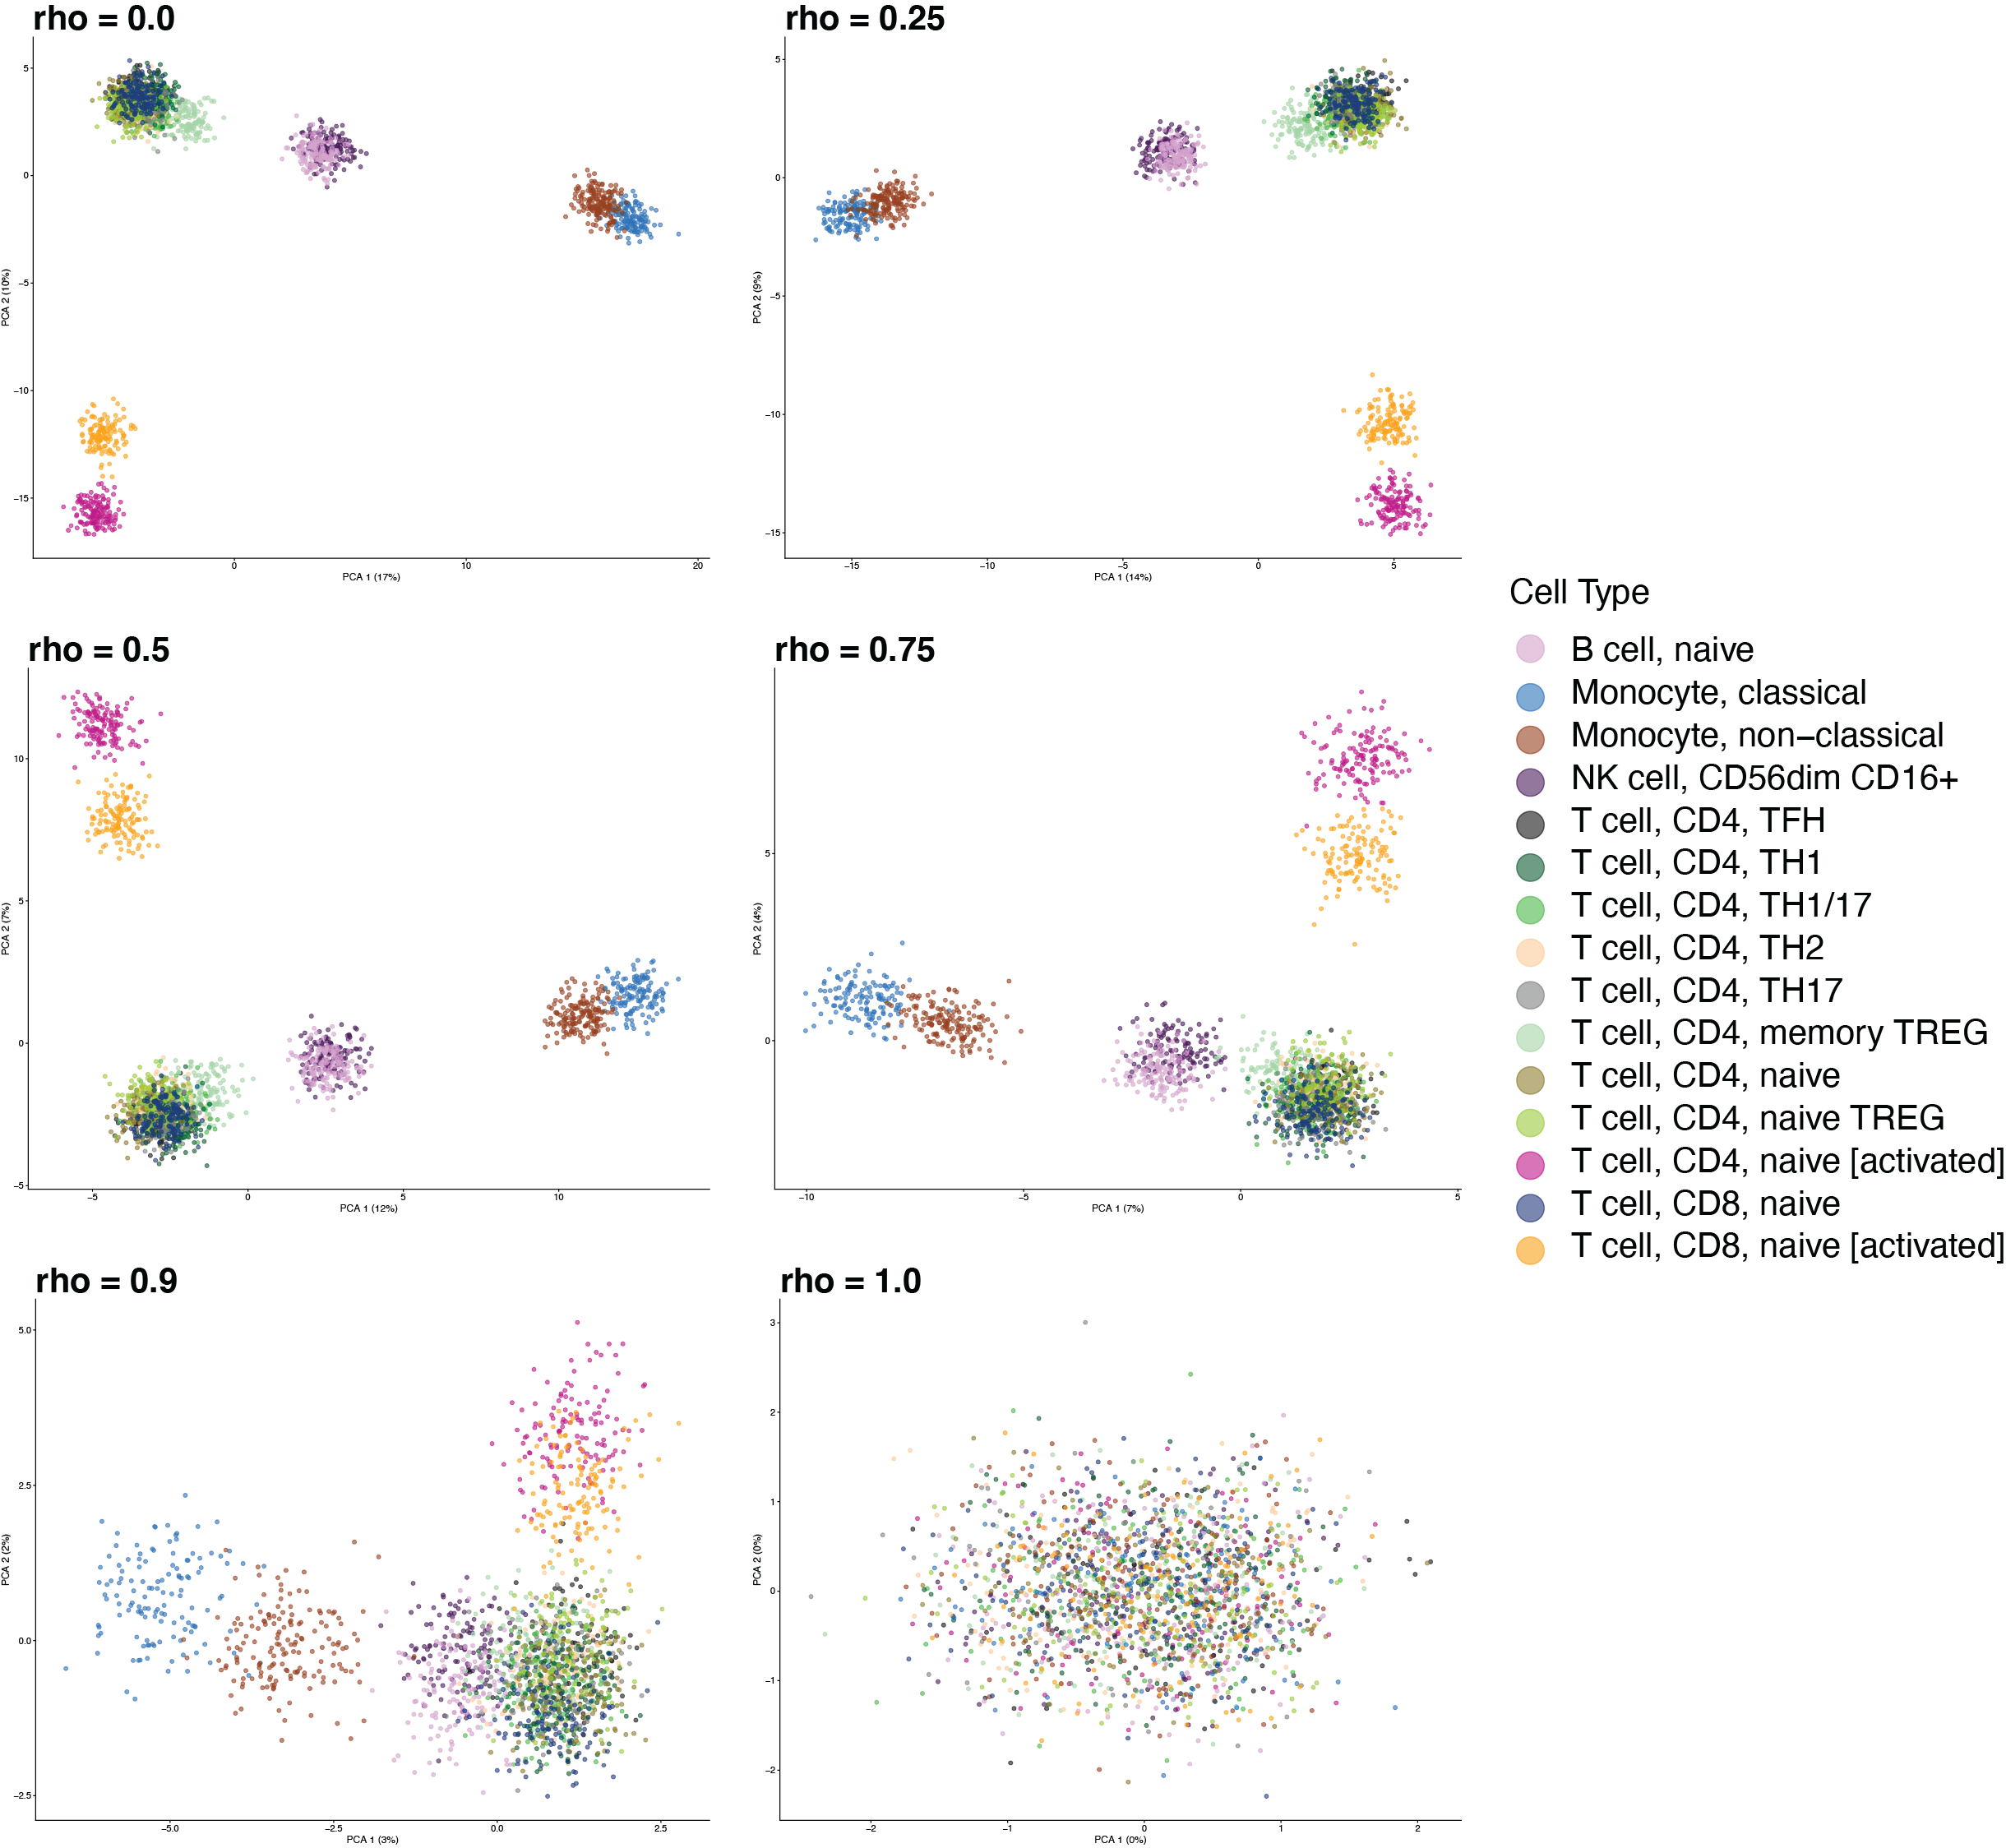
\includegraphics[width=\textwidth]{Figures/sim_data_PCA.png}
    \caption{\textbf{Simulated scRNA-seq datasets exhibit realistic distribution of expression patterns across various noise levels} Shown are the plots of first two PCs for generated immune cell scRNA-seq datasets from the simulation scheme. Datasets generated using various noise proportions $\rho =$ \{0.0, 0.25, 0.5, 0.75, 0.9, 1.0\} are shown and coloured by cell type.}
    \label{fig:ct-pca}
\end{figure}
\subsection{Resulting Simulated Data}
Pseudo scRNA-seq datasets of $N = 2000$ cells and total transcript count $R = 2500$ with varying noise proportions $\rho$ are obtained from the simulation scheme (Fig. \ref{fig:ct-pca}). Total gene count value $R$ is chosen to approximate UMI count values seen in real scRNA-seq data \cite{Hafemeister_2019}. As expected, as $\rho$ is increased, simulated gene expression profiles of immune cell types become less distinct from one another and at $\rho = 1$, the simulated cell population is entirely homogeneous. 

This simulation scheme is able to generate realistic scRNA-seq data that captures the similarities and differences between the given cell types. From the principal component (PC) visualization in the first two PCs, it is seen that classical and non-classical monocytes are distinct from the simulated lymphocyte populations in the first PC (Fig. \ref{fig:ct-pca}). Similarly, activated T cell populations are separated along the second PC. The population of inactivated T cells (CD4+ and CD8+ T cells) are clustered together in the first two PCs suggesting only minor differences in the gene expression profiles of these cells. In the third and fourth PCs, B cells and NK cells distinguish themselves from T cell subsets and each other while T cell subsets begin to separate (Fig. \ref{fig:ct-pca-supp}).

For analysis, a simulated dataset with parameters $\rho = 0.5$ is used. At this $\rho$ value, cell types are still preserved and can be well distinguished while maintaining a level of randomness that accounts for the noise seen in real scRNA-seq samples. 




\subsection{Cell Type Specific Latent Topic Profiles}

\begin{figure}
    \centering
    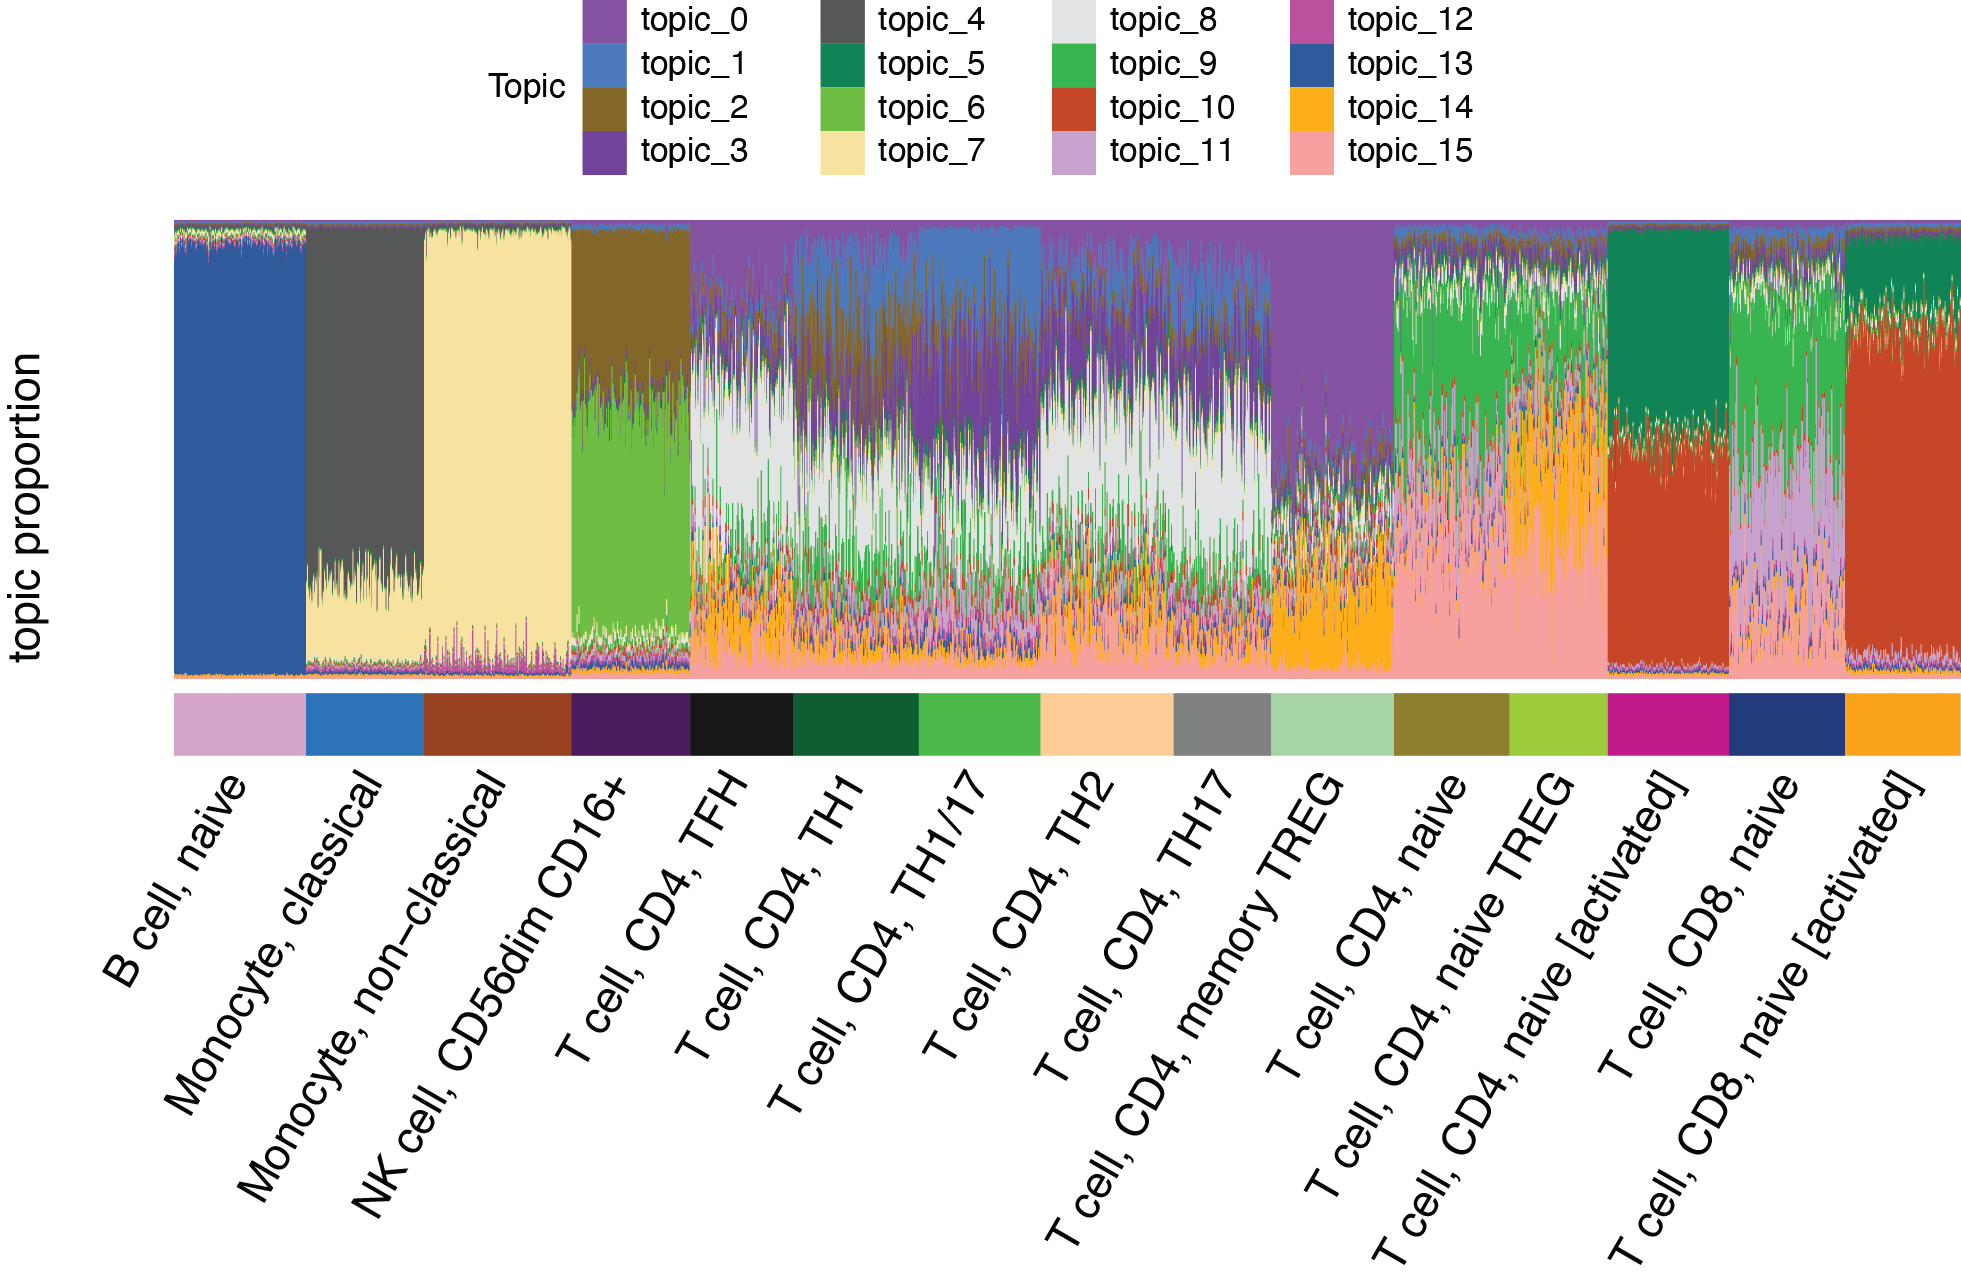
\includegraphics[width=\textwidth]{Figures/structure_plot.png}
    \caption{\textbf{Topic proportions of simulated immune cell gene expression shows distinct latent profiles between cell types} Structure plot of estimated topic proportion $\theta$ values for each cell in the simulated data set. Cells are annotated below by simulated cell type.}
    \label{fig:struct_plt}
\end{figure}

\begin{figure}
    \centering
    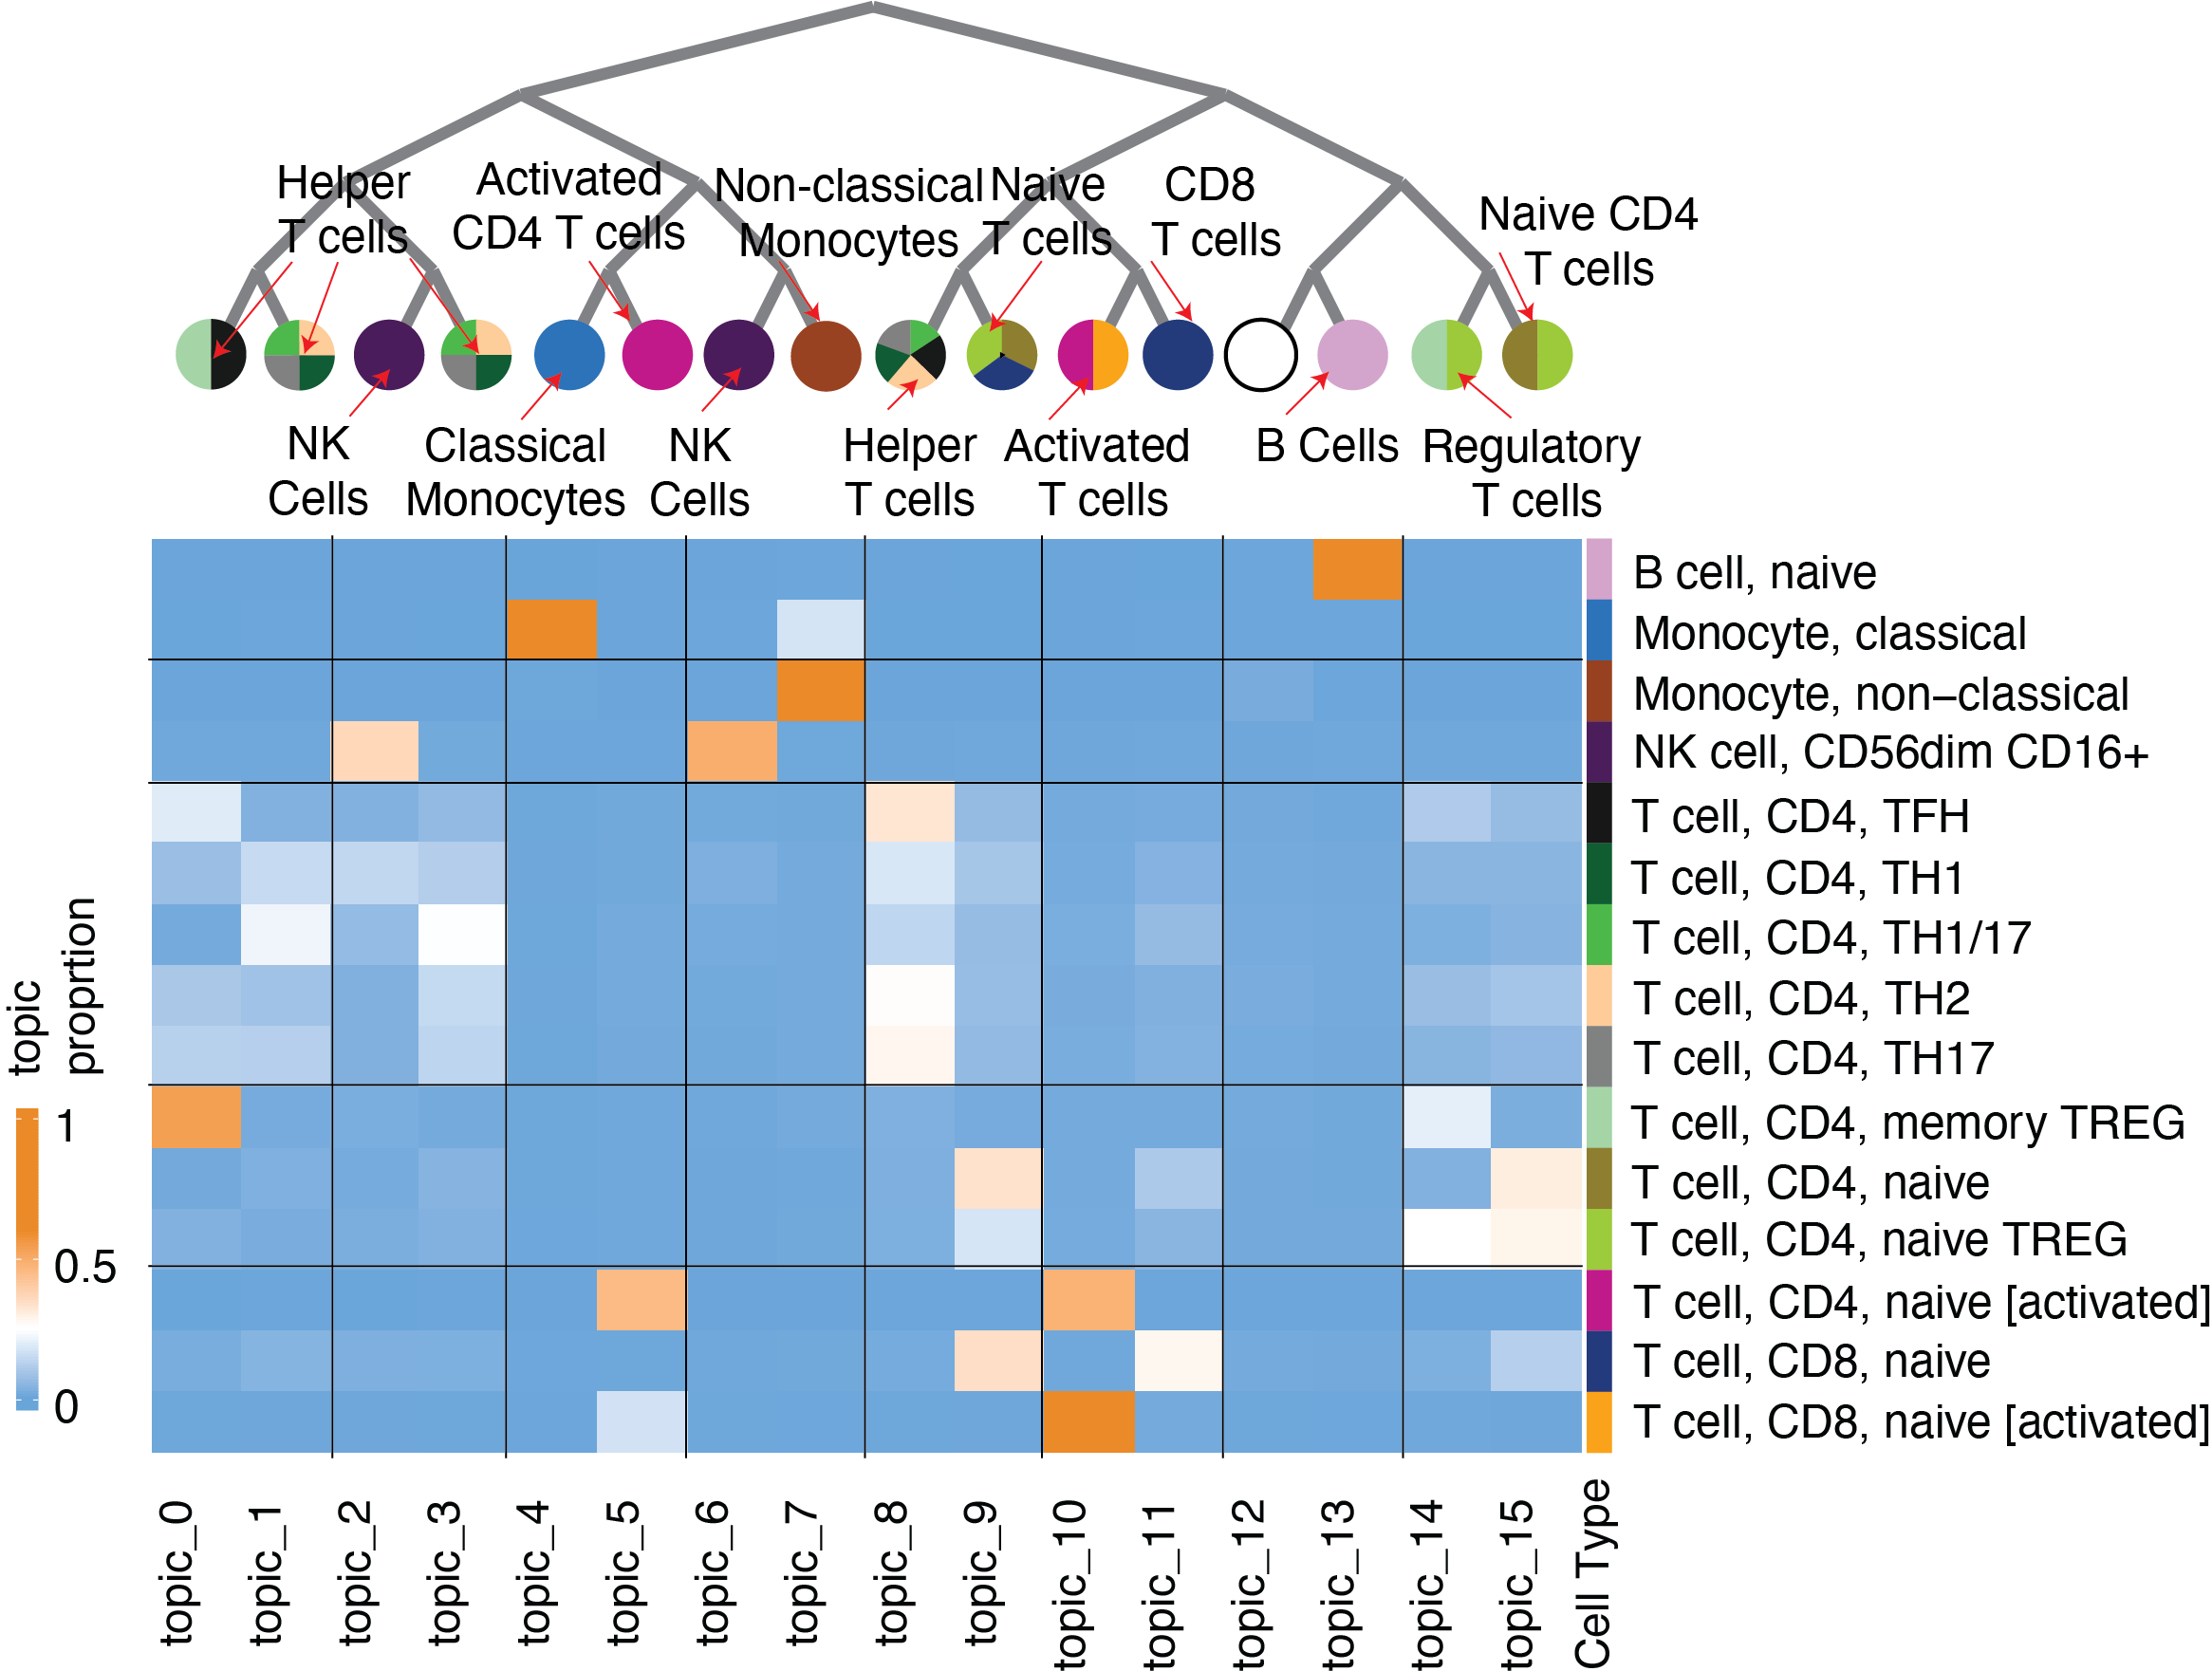
\includegraphics[width=\textwidth]{Figures/hier_hm.png}
    \caption{\textbf{Latent topic profiles can be used to reconstruct tree-structured relationships between cell subsets} The top panel shows the reconstructed tree structure from average latent topic profiles calculated for each cell subset. Below is a heatmap of the mean latent topic proportion profiles across each immune cell subset.}
    \label{fig:hier_hm}
\end{figure}

The LaRCH model was trained on a simulated immune cell scRNA-seq dataset with simulation parameters:
\begin{itemize}
    \item Number of cells $N = 2000$
    \item Noise proportion $\rho = 0.5$
    \item Read depth $R = 2500$
\end{itemize} 
and model parameters:
\begin{itemize}
    \item tree depth $D = 5$
    \item prior inclusion probability $\pi_0 = 0.1$
    \item prior normal variance $\tau_0 = 1$
    \item batch size $|s| = 128$ for $s \in [S]$
    \item learning rate $lr = 0.01$
    \item local KL weight term $kl\_weight = 1.0$
    \item beta KL weight term $kl\_weight\_beta = 1.0$
\end{itemize}

The model is able to recover the simulated cell types and represent each cell subset with a unique topic profile (Fig. \ref{fig:struct_plt}). Biologically similar cell types share topics. This is seen most prominantly amongst helper CD4+ T cell subsets which contain mixtures of topic 1, 3, and 8 (Fig. \ref{fig:hier_hm}). This suggests that the these cell subsets share overlapping expression features. The minor differences in proportions of each topic for each cell subset demonstrates that each helper T cell subset expresses the genetic features captured by each topic to varying levels. Topic 14 is highly represented in regulatory CD4+ T cell subsets, suggesting a regulatory signature being captured in the leaf node within this topic. Similarly, topic 15 is seen in naïve CD4+ T cells, possibly capturing a naïve signature.

Using the topic average latent topic representations of cell subsets, the underlying tree structure is reconstructed qualitatively (Fig. \ref{fig:hier_hm}). Topics with high representation of particular subsets are labeled as a marker topic for said subset. The reconstructed cell hierarchy shares some noticeable similarities to the lineage tree representation of immune cell subsets (Fig. \ref{fig:immune-cells}). 

The latter half of the tree representation contains only cells within the adaptive immune system. Monocytes, which branch from the other subsets at the earliest point in the differentiation process, are solely contained within topics 4 and 7 which share 3 nodes along their paths. Activated CD4+ T cells share a path with classical monocytes, suggesting some activation features captured in their shared nodes. 

Similarly, NK cells, which are involved in both innate and adaptive immune function, are represented in topic 7, sharing a node path with non-classical monocytes and it is likely that innate immune response gene signatures are captured within their shared paths, especially in nodes 4 and 10 which are not shared by any other subsets. NK cells are also represented by topic 2 which shares a node path with topic 3 which represents a number of helper T cell subsets. The shared nodes between these topics (nodes 1, 3, 8) likely contain gene embeddings related to adaptive immune response.

Topics 8 through 11 solely represent T cell subsets, capturing overlapping T lymphocyte gene expression patterns. More distinct cell types are contained within unique branches of the tree, such as B cells which are the only cell type represented in the branch containing topics 12 and 13.

Topic 14 captures features of regulatory T cell subsets which topic 15 captures those of naïve CD4+ T cells. This suggests that the nodes that constitute the shared path between these two topics (nodes 0, 2, 6, and 14) contain embeddings of genes related to CD4+ T cell function that are shared between all these T cell subsets, while node 29, the leaf node of topic 14 contains gene embeddings related to regulatory function and node 30, the leaf node of topic 15 is related to naïve expression profiles. 



\subsection{Using Latent Features in Place of Other Dimensionality Reduction Techniques for Downstream Analysis}
\begin{figure}
    \centering
    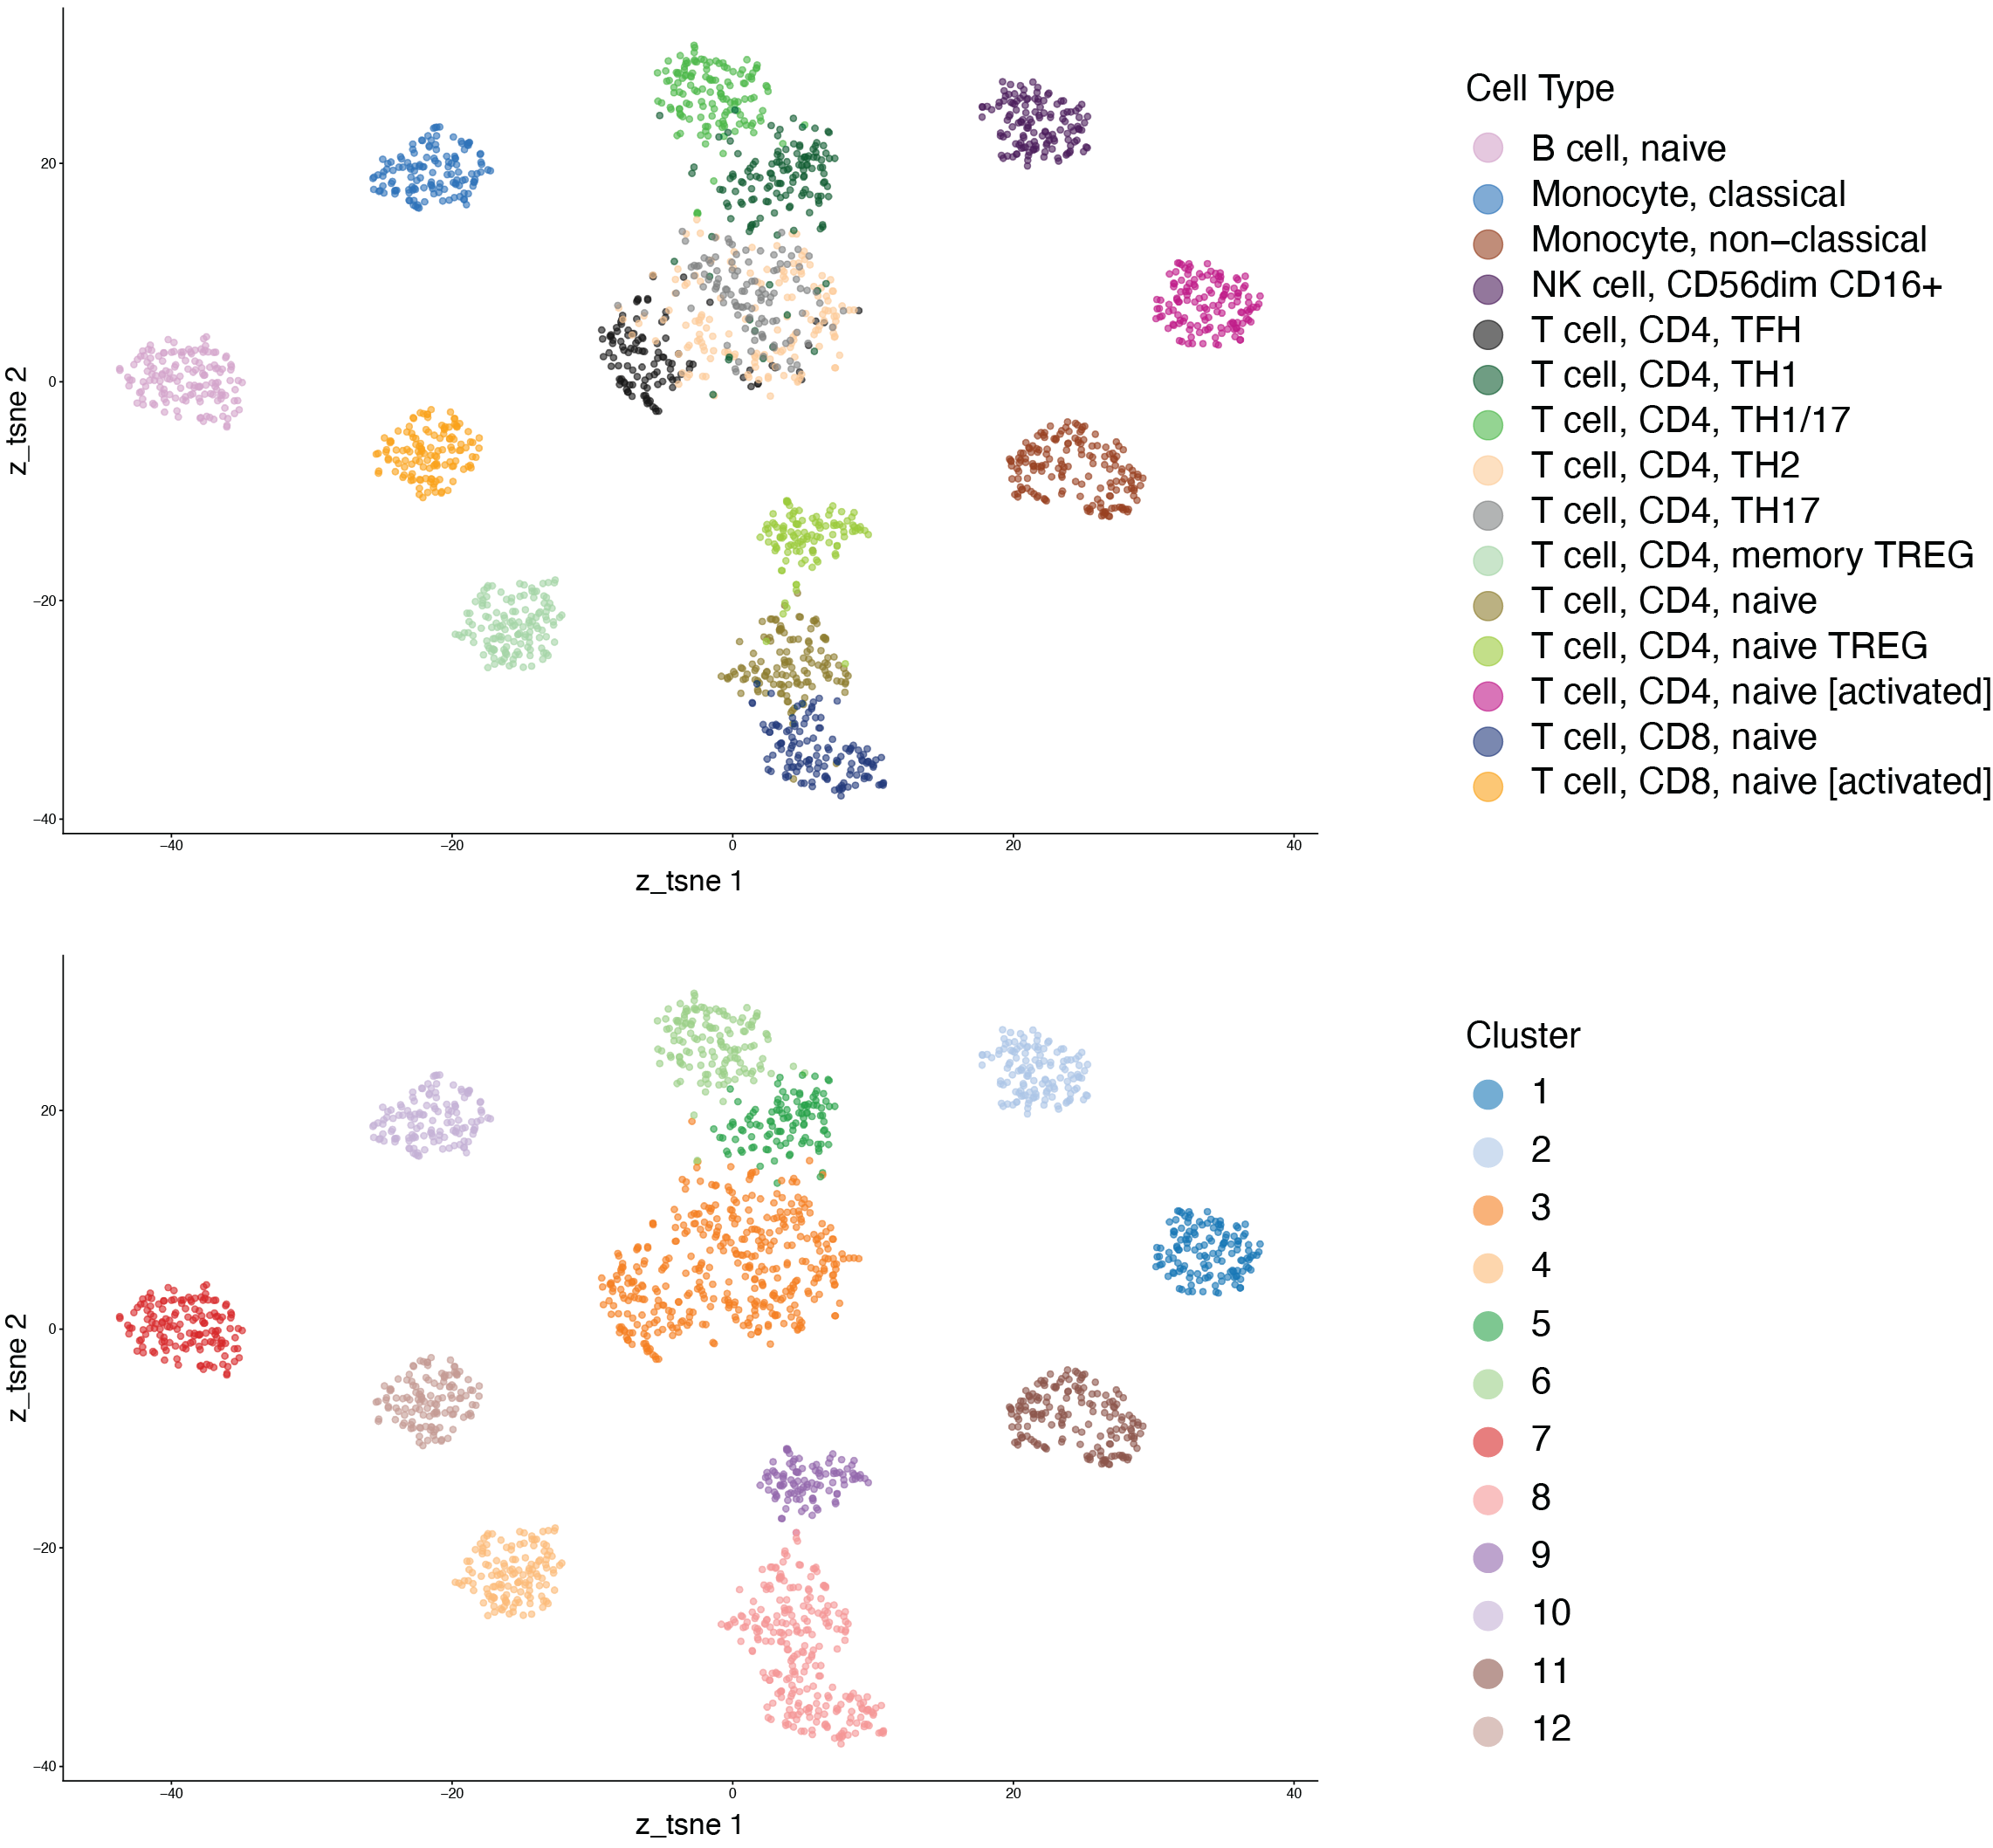
\includegraphics[width=\textwidth]{Figures/cluster_tsne.png}
    \caption{\textbf{Louvain lustering on latent topic space recovers groups of cells corresponding to their simulated cell type} The top panel shows the simulated cells in tSNE space coloured by original simulated cell type. The bottom panel shows the clusters generated using louvain clustering on the latent topic representation of cells. For visualization, tSNE dimensions were generated from the latent topic space.}
    \label{fig:sim_clusters}
\end{figure}

To test the efficacy of the LaRCH model and its ability to perform cell type deconvolution from single-cell gene expression data, clustering was performed using the latent topic features estimated from simulated data. 

The Louvain method of community detection \cite{louvain} was used to extract cell type clusters from a K-nearest neighbour graph ($k = 10$ was used) constructed using the latent topic features to calculate distance between data points. In general, the resulting cell clusters separate the various simulated cell types, missing only some granularity between closely related cell types (Fig. \ref{fig:sim_clusters}). In this case, the clustering done is unable to distinguish between certain subsets of T cells. The helper T cell subsets of T follicular helpers, Th17s, and Th2s are all contained within cluster 3 from figure \ref{fig:sim_clusters}, it is seen that these cells lie closely in the t-distributed stochastic neighbor embedding (tSNE) reduced dimension space, showing that the simulated transcriptional profiles of these cell are very similar. Additionally, cluster 8 contains the naïve subsets of both CD4+ and CD8+ cell types. The grouping of these cell types within the latent feature space suggests an overlap in overall gene expression profile and cellular function between cell types. Changing Louvain clustering parameters ($k = 5$) creates a more granular clustering that more accurately separates individual cell types, but this also runs the risk of over-clustering. 

\begin{figure}
    \centering
    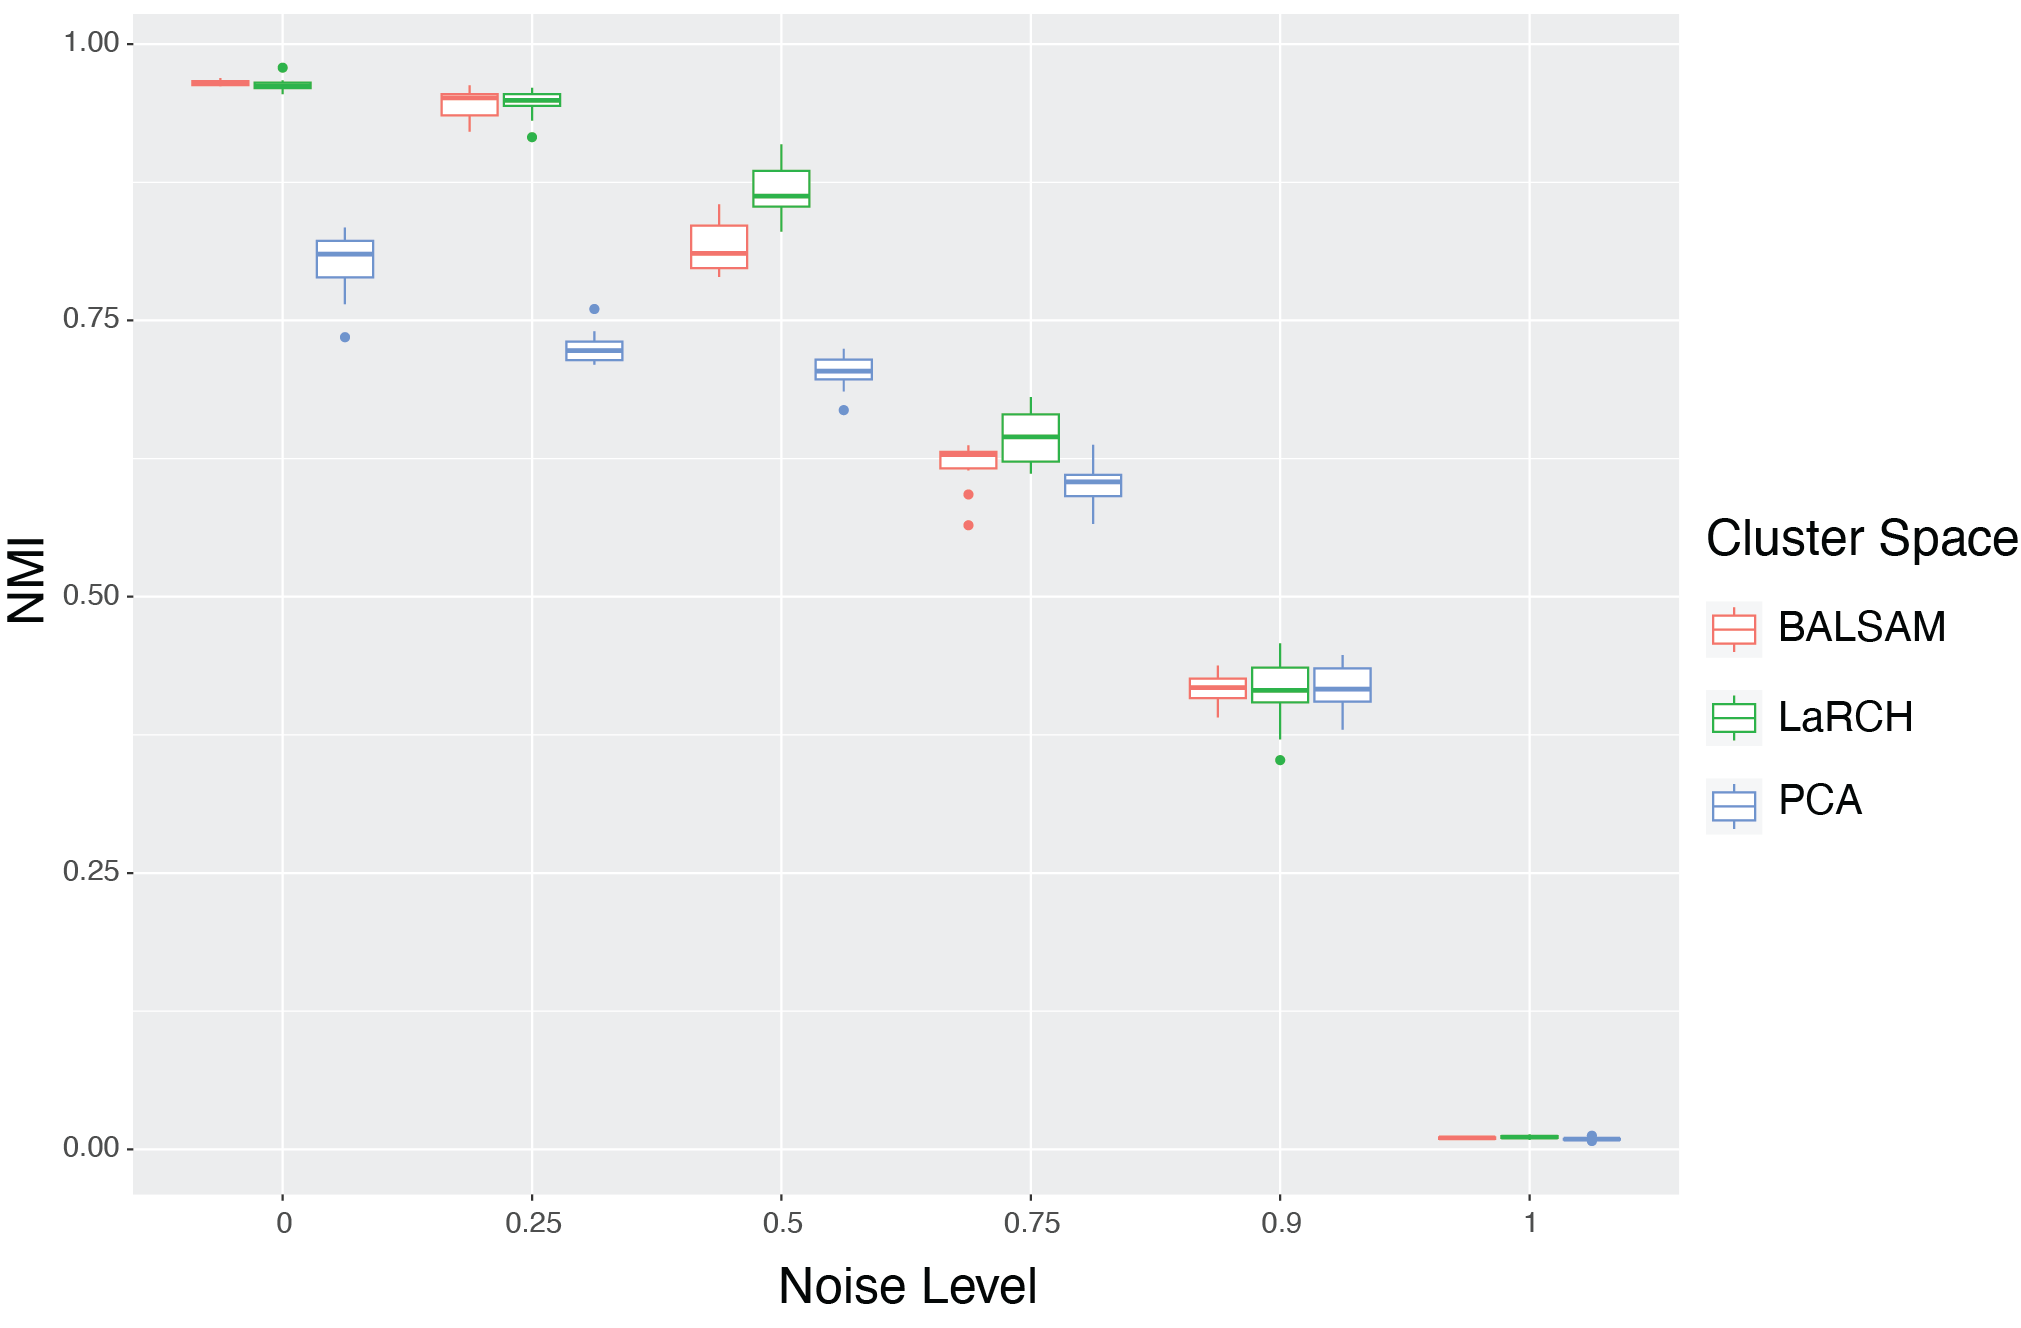
\includegraphics[width=\textwidth]{Figures/nmi_comp.png}
    \caption{\textbf{Using the LaRCH latent space for clustering consistently outperforms clustering on PCA and flat latent topic space} NMI calculated from clustering results from each dimensionality reduction technique and the original simulated cell types across various noise levels. At each noise level, 10 datasets were simulated with different starting seeds.}
    \label{fig:nmi}
\end{figure}

Clustering results from latent topic features as the clustering space were compared to clusters obtained from the first 50 PCs as well as BALSAM \cite{ZHANG2023100388} with 16 latent topics, the same number of latent topics as a LaRCH model with depth $D = 5$. BALSAM is a comparable ETM that utilizes the same encoder-decoder scheme as LaRCH without the underlying tree structure. At each noise level ($\rho =$ 0, 0.25, 0.5, 0.75, 0.9, 1), 10 datasets were simulated with different starting seeds. The Louvain method of community detection \cite{louvain} was then used to detect clusters from the K-nearest neighbour graphs ($k = 10$ was used) constructed from each reduced dimension space. The normalized mutual information (NMI) was calculated from each clustering result and original simulated cell types to compare clustering accuracy (Fig. \ref{fig:nmi}). 

At all noise proportions, clustering from the LaRCH latent feature space outperforms PCA clusters. At low noise proportions, BALSAM and LaRCH are comparable in NMI while at mid-level noise proportions ($rho = 0.5$ and $\rho = 0.75$), LaRCH performs slightly better than BALSAM, showing that the underlying tree-structure provides additional insight on cell type features to the latent topics that are not captures in a flat model. At $rho = 0.9$, where the simluated data is primarily noise and no longer realistic in its representation of a real scRNA-seq dataset, the NMI drops below 0.5 and all clustering methods struggle. 

